\section{Estudo pré-laboratorial}
\subsection{Princípio da Superposição e Conversores D/A}


Os sinais elétricos podem ser descritos genericamente como estando nas formas analógica ou digital. Um sinal analógico é contínuo tanto no tempo quanto na amplitude. Como exemplo, pode-se citar um sinal de uma gravação de música na saída de um amplificador de áudio que alimenta um alto-falante. Por outro lado, um sinal digital, tipicamente representado por números binários, corresponde a uma representação por amostras do sinal analógico original. As amostras do sinal digital podem assumir valores discretos (isto é, um número finito de valores) e representam o sinal em instantes de tempo discretos (em instantes de tempo definidos). Assim, um número binário pode corresponder a um determinado valor de tensão em um determinado instante de tempo. A Fig. 2.1 ilustra o processo de digitalização de um sinal de áudio. Primeiramente, os valores de tensão do sinal analógico (Fig. 2.1a) são tomados a intervalos regulares de tempo, resultando no sinal amostrado (Fig. 2.1b). Depois, o sinal amostrado é quantizado (Fig. 2.1c), ou seja, cada valor de tensão do sinal amostrado será substituído por um dos 2n valores de tensão possíveis, onde n é o número de bits que irão representar cada amostra. Por fim, o sinal quantizado é convertido em uma sequência de bits, onde cada grupo de bits corresponde a um dos valores possíveis no processo de quantização (Fig. 2.1d). Um problema importante em engenharia eletrônica é o uso de um circuito para a conversão de um sinal da forma digital para a forma analógica. O circuito poderia ser usado, por exemplo, em um aparelho de CD. Um número binário (formado por zeros e uns) — correspondente a uma amostra do sinal original, gravado no CD — deve ser convertido para um valor de tensão, que vai representar uma aproximação do sinal analógico durante um intervalo de tempo definido. Um circuito para converter de digital para analógico é apresentado na Fig. 2.2. Cada um dos bits do número binário está associado a um conjunto formado por uma bateria e uma chave. Quando o valor do bit é igual a 1 , a chave correspondente é conectada à bateria; quando o valor é igual a 0 , a chave é conectada ao terra do circuito. A posição da chave é controlada pelo valor do bit. Desta forma, um número binário 000 faz aparecer uma tensão V o = 0 V , enquanto que o número 111 faz aparecer uma tensão V o = 7 / 12 V bat . No circuito, cada número binário entre 000 e 111 corresponde a um valor de tensão que vai representar uma amostra do sinal durante um intervalo de tempo determinado. Por exemplo, para obter uma forma de onda do tipo rampa na saída V o , bastaria escrever em sequência as palavras binárias que vão de 000 a 111 , em incrementos de 1 . Um conversor D/A com mais bits pode ser obtido simplesmente acrescentando novos pares de resistores R-2R e novas chaves ao circuito.
\begin{figure}[H] 
  \centering 
  \begin{subfigure}{.33\textwidth}
    \centering
    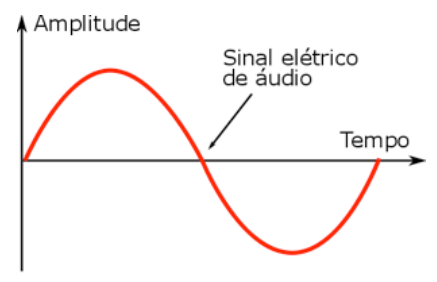
\includegraphics[width=.5\textwidth]{imagens/pdf_images/a.png}
    \caption{}
    \label{fig:a_sf}
  \end{subfigure}
  \begin{subfigure}{.33\textwidth}
    \centering
    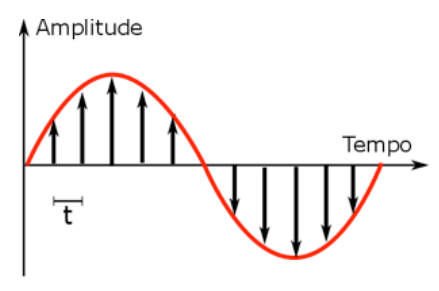
\includegraphics[width=.5\textwidth]{imagens/pdf_images/b.png}
    \caption{}
    \label{fig:b_sf}
  \end{subfigure}
  \begin{subfigure}{.33\textwidth}
    \centering
    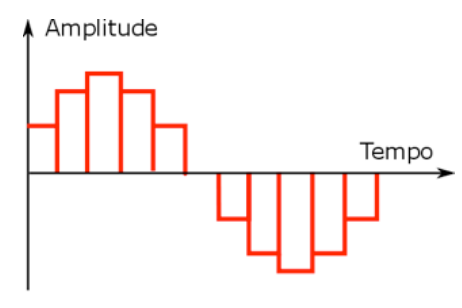
\includegraphics[width=.5\textwidth]{imagens/pdf_images/c.png}
    \caption{}
    \label{fig:c_sf}
  \end{subfigure}
  
  \begin{subfigure}{.33\textwidth}
    \centering
    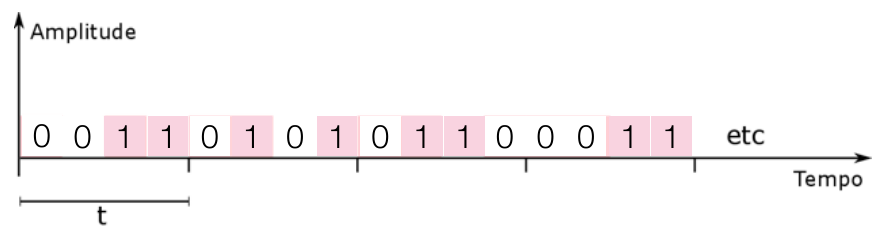
\includegraphics[width=1.3\textwidth]{imagens/pdf_images/d.png}
    \caption{}
    \label{fig:d_sf}
  \end{subfigure}
  
  
  \caption{Conversão analógico-digital (A/D): (a) sinal analógico; (b) discretização no tempo (amostragem); (c) discretização em amplitude (quantização); e (d) representação do sinal digital na forma de bits.}
  \label{fig:fig1}
\end{figure}

\begin{figure}[H]
  \centering
  \begin{circuitikz}[line width = .5pt, scale = .8, transform shape, american voltages]
    \draw
      (0,0) node [ground] {} -- (0,.5)
      to [short] (5,.5) to [R,l=$2R$] (5,8) -- (3,8)
      to [R,l=$R$, *-] (0,8) to [R,l=$R$, *-*] (-3,8) -- (-5,8) -- (-5,5)
      to [R, l=$2R$, v=$V_o$] (-5, 3) -- (-5,.5) -- (0,.5);
    \draw
    (-3,8) to [R,l=$2R$] (-3,5.5);
    \draw
    (-3,5)  node [spdt, rotate = -90] (Sw){}
    (Sw.out 2) to [short, -*] ($(Sw.out 2)-(0,3.9)$); 
    \draw
    (-2.5,5) node [right] {bit2};
    \draw
    (3,5)  node [spdt, rotate = -90] (Sw3){}
    (Sw3.out 1) to [short, -*] ($(Sw3.out 1)-(0,3.9)$); 
    \draw
    (3,8) to [R, l=$2R$] (3,5.5); 
    \draw
    ($(Sw.out 1) - (0,.5)$) -- ($(Sw3.out 2)-(0,.5)$);
    \draw
    (Sw.out 1) -- ($(Sw.out 1) - (0,.5)$) to [short, -*] (.3,3.9) -- 
    ($(Sw3.out 2) - (0,.5)$)--(Sw3.out 2);
    \draw
    (0,8) to [R, l=$2R$] (0,5.5);
    \draw
    (0,5) node [spdt, rotate = -90] (Sw2) {};
    \draw
    (1.5,5) node [left] {bit1};
    \draw 
    (.3,.5) to [battery, v_<=$Vbat$, *-]  (Sw2.out 1);
    \draw
    (Sw2.out 2) -- ($(Sw2.out 2) -(.5,0)$) -- (-.8,.5);
    \draw
    (4.5,5) node [left] {bit0};
    
  \end{circuitikz}
  \caption{Conversor Digital-Analógico (D/A) tipo rede R-2R de 3 bits.}
  \label{circ:conv_da}
\end{figure}

\subsubsection{Por meio de análise teórica do circuito da Fig. 2.2, encontre o valor da saída V o para cada uma das 8 palavras binárias de 3 bits possíveis ( 000 a 111 ). Para tal, considere $V_{bat}$ = 5 V.}


\noindent Dica: ao invés de resolver o circuito oito vezes, resolva apenas para as palavras binárias 000, 001, 010 e 100. A seguir, aplique o teorema da superposição para encontrar o resultado para as demais palavras binárias 


\noindent \textbf{a)} Para a palavra binária 000, tem-se o seguinte circuito:


\begin{figure}[H]
  \centering
  \begin{circuitikz}[line width = .5pt, scale = .8, transform shape, american voltages]
    \draw
      (0,0) node [ground] {} -- (0,.5)
      to [short] (5,.5) to [R,l=$2R$] (5,8) -- (3,8)
      to [R,l=$R$, *-] (0,8) to [R,l=$R$, *-*] (-3,8) -- (-5,8) -- (-5,5)
      to [R, l=$2R$, v=$V_o$] (-5, 3) -- (-5,.5) -- (0,.5);
    \draw
    (-3,8) node [above, color=red] {A} to [R,l=$2R$] (-3,5.5);
    \draw
    (-3,5)  node [spdt, rotate = 90, xscale=-1] (Sw){}
    (Sw.out 1) to [short, -*] ($(Sw.out 1)-(0,3.9)$); 
    \draw
    (-2.5,5) node [right] {bit2};
    \draw
    (3,5)  node [spdt, rotate =-90, xscale=1] (Sw3){}
    (Sw3.out 1) to [short, -*] ($(Sw3.out 1)-(0,3.9)$); 
    \draw
    (3,8) node [above, color=red] {C} to [R, l=$2R$] (3,5.5); 
    \draw 
    (Sw.out 2) -- ($(Sw.out 2) - (0,.5)$) to [short, -*] (.3,3.9) -- 
    ($(Sw3.out 2) - (0,.5)$)--(Sw3.out 2);
    \draw
    (0,8) node [above, color=red] {B} to [R, l=$2R$] (0,5.5);
    \draw
    (0,5) node [spdt, rotate = 90, xscale=-1] (Sw2) {};
    \draw
    (1.5,5) node [left] {bit1};
    \draw 
    (.3,.5) to [battery, v_<=$Vbat$, *-]  (Sw2.out 2);
    \draw
    (Sw2.out 1) -- ($(Sw2.out 1) -(.5,0)$) -- (-.8,.5);
    \draw
    (4.5,5) node [left] {bit0};
    
  \end{circuitikz}
  \caption{Conversor Digital-Analógico (D/A) tipo rede R-2R de 3 bits.}
  \label{circ:conv_da}
\end{figure}


Como não há participação da fonte (bateria), então o valor de $V_o=V_{000}=0V$.

\textbf{b)} Para a palavra binária 001, tem-se o seguinte resultado:

\begin{figure}[H]
  \centering
  \begin{circuitikz}[line width = .5pt, scale = .8, transform shape, american voltages]
    \draw
      (0,0) node [ground] {} -- (0,.5)
      to [short] (5,.5) to [R,l=$2R$] (5,8) -- (3,8)
      to [R,l=$R$, *-] (0,8) to [R,l=$R$, *-*] (-3,8) -- (-5,8) -- (-5,5)
      to [R, l=$2R$, v=$V_o$] (-5, 3) -- (-5,.5) -- (0,.5);
    \draw
    (-3,8) node [above, color=red] {A} to [R,l=$2R$] (-3,5.5);
    \draw
    (-3,5)  node [spdt, rotate = 90, xscale=-1] (Sw){}
    (Sw.out 1) to [short, -*] ($(Sw.out 1)-(0,3.9)$); 
    \draw
    (-2.5,5) node [right] {bit2};
    \draw
    (3,5)  node [spdt, rotate =90, xscale=-1] (Sw3){}
    (Sw3.out 2) to [short, -*] ($(Sw3.out 2)-(0,3.9)$); 
    \draw
    (3,8) node [above, color=red] {C} to [R, l=$2R$] (3,5.5); 
    \draw 
    (Sw.out 2) -- ($(Sw.out 2) - (0,.5)$) to [short, -*] (.3,3.9) -- 
    ($(Sw3.out 1) - (0,.5)$)--(Sw3.out 1);
    \draw
    (0,8) node [above, color=red] {B} to [R, l=$2R$] (0,5.5);
    \draw
    (0,5) node [spdt, rotate = 90, xscale=-1] (Sw2) {};
    \draw
    (1.5,5) node [left] {bit1};
    \draw 
    (.3,.5) to [battery, v_<=$Vbat$, *-]  (Sw2.out 2);
    \draw
    (Sw2.out 1) -- ($(Sw2.out 1) -(.5,0)$) -- (-.8,.5);
    \draw
    (4.5,5) node [left] {bit0};
    
  \end{circuitikz}
  \caption{Conversor Digital-Analógico (D/A) tipo rede R-2R de 3 bits.}
  \label{circ:conv_da}
\end{figure}

Aplicando a LKT, temos
\[
\begin{cases}
  \dfrac{V_A - V_B}{R} + \dfrac{V_A}{2R}=0\\
  \\
  \dfrac{V_B - V_A}{R} + \dfrac{V_B}{2R} + \dfrac{V_B - V_C}{R}=0\\
  \\
  \dfrac{V_C - V_B}{R} + \dfrac{V_C - 5}{2R} + \dfrac{V_C}{2R}=0
\end{cases}
\rightarrow
\begin{cases}
  2V_A-V_B+0V_C=0\\
  -1V_A + 2,5V_B-1V_C=0\\
  0V_A-1V_b+2V_C=0
\end{cases}
\]

Transpondo o sistema de equações obtido acima para uma matriz $3x3$, temos

\[
\begin{bmatrix}
  2 & -1 & 0\\
  -1 & 2,5 & -1\\
  0 & -1 & 2
\end{bmatrix}
\cdot
\begin{bmatrix}
  V_A\\
  V_B\\
  V_C
\end{bmatrix}
=
\begin{bmatrix}
  0\\0\\0
\end{bmatrix}
\]

Resolvendo a matriz encontramos
\[
  \begin{cases}
    V_A=0,4167\\V_B=0,8333\\V_C=1,6667
  \end{cases}
\]

Logo, 

\begin{equation}
  V_A=V_o=V_{001}=0,4167V
\end{equation}

\textbf{c)} Para a palavra binária 010, temos a seguinte configuração


\begin{figure}[H]
  \centering
  \begin{circuitikz}[line width = .5pt, scale = .8, transform shape, american voltages]
    \draw
      (0,0) node [ground] {} -- (0,.5)
      to [short] (5,.5) to [R,l=$2R$] (5,8) -- (3,8)
      to [R,l=$R$, *-] (0,8) to [R,l=$R$, *-*] (-3,8) -- (-5,8) -- (-5,5)
      to [R, l=$2R$, v=$V_o$] (-5, 3) -- (-5,.5) -- (0,.5);
    \draw
    (-3,8) node [above, color=red] {A} to [R,l=$2R$] (-3,5.5);
    \draw
    (-3,5)  node [spdt, rotate = 90, xscale=-1] (Sw){}
    (Sw.out 1) to [short, -*] ($(Sw.out 1)-(0,3.9)$); 
    \draw
    (-2.5,5) node [right] {bit2};
    \draw
    (3,5)  node [spdt, rotate =-90, xscale=1] (Sw3){}
    (Sw3.out 1) to [short, -*] ($(Sw3.out 1)-(0,3.9)$); 
    \draw
    (3,8) node [above, color=red] {C} to [R, l=$2R$] (3,5.5); 
    \draw 
    (Sw.out 2) -- ($(Sw.out 2) - (0,.5)$) to [short, -*] (.3,3.9) -- 
    ($(Sw3.out 2) - (0,.5)$)--(Sw3.out 2);
    \draw
    (0,8) node [above, color=red] {B} to [R, l=$2R$] (0,5.5);
    \draw
    (0,5) node [spdt, rotate =-90, xscale=1] (Sw2) {};
    \draw
    (1.5,5) node [left] {bit1};
    \draw 
    (.3,.5) to [battery, v_<=$Vbat$, *-]  (Sw2.out 1);
    \draw
    (Sw2.out 2) -- ($(Sw2.out 2) -(.5,0)$) -- (-.8,.5);
    \draw
    (4.5,5) node [left] {bit0};
    
  \end{circuitikz}
  \caption{Conversor Digital-Analógico (D/A) tipo rede R-2R de 3 bits.}
  \label{circ:conv_da}
\end{figure}

Aplicando a LKT, temos

\[
  \begin{cases}
    \dfrac{V_A - V_B}{R} + \dfrac{V_A}{2R} + \dfrac{V_A}{2R} =0\\
    \\
    \dfrac{V_B - V_A}{R} + \dfrac{V_B - 5}{2R} + \dfrac{V_B - V_C}{R}  =0\\
    \\
    \dfrac{V_C - V_B}{R} + \dfrac{V_C}{2R} + \dfrac{V_C}{2R} =0
  \end{cases}
  \rightarrow
  \begin{cases}
    2V_A - 1V_B + 0V_C = 0  \\
    -1V_A + 2,5V_B - 1V_C=2,5\\
    0V_A-1V_B+2V_C=0
  \end{cases}
\]

Colocando em forma matricial, tem-se

\[
  \begin{bmatrix}
    2 & -1 & 0\\
    -1 & 2,5 & -1 \\
    0 & -1 & 2
  \end{bmatrix}
  \cdot 
  \begin{bmatrix}
    V_A\\V_B\\V_C
  \end{bmatrix}
  =
  \begin{bmatrix}
    0\\2,5\\0
  \end{bmatrix}
\]

Resolvendo a matriz, obtem-se

\[
  \begin{cases}
    V_A=0,8333V\\V_B=1,6667V\\V_C=0,8333V
  \end{cases}
\]
Logo,

\begin{equation}
  V_A=V_o=V_{010}=0,8333V
\end{equation}

\textbf{d)} Para a palavra 100, tem-se o seguinte circuito


\begin{figure}[H]
  \centering
  \begin{circuitikz}[line width = .5pt, scale = .8, transform shape, american voltages]
    \draw
      (0,0) node [ground] {} -- (0,.5)
      to [short] (5,.5) to [R,l=$2R$] (5,8) -- (3,8)
      to [R,l=$R$, *-] (0,8) to [R,l=$R$, *-*] (-3,8) -- (-5,8) -- (-5,5)
      to [R, l=$2R$, v=$V_o$] (-5, 3) -- (-5,.5) -- (0,.5);
    \draw
    (-3,8) node [above, color=red] {A} to [R,l=$2R$] (-3,5.5);
    \draw
    (-3,5)  node [spdt, rotate =-90, xscale=1] (Sw){}
    (Sw.out 2) to [short, -*] ($(Sw.out 2)-(0,3.9)$); 
    \draw
    (-2.5,5) node [right] {bit2};
    \draw
    (3,5)  node [spdt, rotate =-90, xscale=1] (Sw3){}
    (Sw3.out 1) to [short, -*] ($(Sw3.out 1)-(0,3.9)$); 
    \draw
    (3,8) node [above, color=red] {C} to [R, l=$2R$] (3,5.5); 
    \draw 
    (Sw.out 1) -- ($(Sw.out 1) - (0,.5)$) to [short, -*] (.3,3.9) -- 
    ($(Sw3.out 2) - (0,.5)$)--(Sw3.out 2);
    \draw
    (0,8) node [above, color=red] {B} to [R, l=$2R$] (0,5.5);
    \draw
    (0,5) node [spdt, rotate =90, xscale=-1] (Sw2) {};
    \draw
    (1.5,5) node [left] {bit1};
    \draw 
    (.3,.5) to [battery, v_<=$Vbat$, *-]  (Sw2.out 2);
    \draw
    (Sw2.out 1) -- ($(Sw2.out 1) -(.5,0)$) -- (-.8,.5);
    \draw
    (4.5,5) node [left] {bit0};
    
  \end{circuitikz}
  \caption{Conversor Digital-Analógico (D/A) tipo rede R-2R de 3 bits.}
  \label{circ:conv_da}
\end{figure}

Aplicando a LKT, tem-se

\[
  \begin{cases}
    \dfrac{V_A - V_B }{R} + \dfrac{V_A - 5}{2R} + \dfrac{V_A}{2R} =0\\
    \\
    \dfrac{V_B-V_A}{R} + \dfrac{V_B}{2R} + \dfrac{V_B-V_C}{R} =0\\
    \\
    \dfrac{V_C-V_B}{R} + \dfrac{V_C}{2R} + \dfrac{V_C}{2R} =0
  \end{cases}
  \rightarrow
  \begin{cases}
    2V_A -1V_B + 0V_C=2,5\\
    -1V_A+2,5V_B-1V_C=0\\
    0V_A-1V_B+2V_C=0
  \end{cases}
\]

Arranjando o sistema de equações de forma matricial, tem-se

\[
  \begin{bmatrix}
    2 & -1 & 0\\
    -1 & 2,5 & -1\\
    0 & -1 & 2
  \end{bmatrix}
  \cdot
  \begin{bmatrix}
    V_A\\V_B\\V_C
  \end{bmatrix}
  =
  \begin{bmatrix}
    2,5\\0\\0
  \end{bmatrix}
\]

Como resultado, obtem-se

\[
  \begin{cases}
    V_A=1,6667V\\V_B=0,8333V\\V_C=0,4167V
  \end{cases}
\]
Logo,
\begin{equation}
  V_A=V_o=V_{100}=1,6667V
\end{equation}

\textbf{e)} Aplicando-se o teorema da superposição, se pode encontrar os valores em volts das demais palavras binárias. Assim

\[
  \begin{cases}
    V_{011}=V_{001}+V_{010}=0,4167+0,8333=1,25V\\
    V_{101}=V_{100}+V_{001}=1,6667+0,4167=2,0834V\\
    V_{110}=V_{010}+V_{100}=0,8333+1,6667=2,5V\\
    V_{111}=V_{001}+V_{010}+V_{100}=0,4167+0,8333+1,6667=2,9167V
  \end{cases}
\]

\noindent\textbf{b)} Verifique os resultados teóricos encontrados, simulando o circuito no Qucs 0.0.19. Obtenha os valores da saída $V_o$ correspondentes a cada uma das entradas possíveis ( 000 a 111 ).

\figuras{.5}{imagens/DA/param_diagram.png}{<++>}{<++>}
\figuras{.5}{imagens/DA/new_sch.png}{<++>}{<++>}
\figuras{.5}{imagens/DA/v000.png}{<++>}{<++>}
\figuras{.5}{imagens/DA/final_circuits_da.png}{<++>}{<++>}
\figuras{.5}{imagens/DA/circuits_da.png}{<++>}{<++>}
\figuras{.5}{imagens/DA/ins_dc_sim.png}{<++>}{<++>}
\figuras{.5}{imagens/DA/ins_dc.png}{<++>}{<++>}
\figuras{.5}{imagens/DA/ins_res.png}{<++>}{<++>}
